\documentclass{standalone}
\usepackage{amsfonts,amsmath,amssymb}
\usepackage[slovene]{babel}
\usepackage[utf8]{inputenc}
\usepackage[T1]{fontenc}
  
\usepackage{tikz, verbatim}
\usepackage{pgfplots}
\usetikzlibrary{arrows.meta, calc, positioning, automata}

\begin{document}

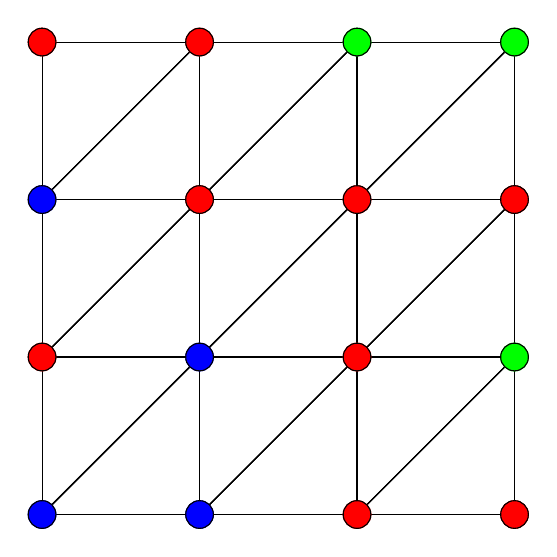
\begin{tikzpicture}
		\foreach \x in {0,2,4,6}
		{   \foreach \y in {0,2,4,6}
		    {  \fill (\x,\y) circle (5pt);
		       \draw (0, \y ) -- (6, \y );
		       \draw (\x ,0) -- (\x ,6);
		       \draw ( 0 , \x) -- ( 6 - \x ,6);
		       \draw ( \x , 0) -- ( 6 ,6 - \x );
		    }
		}			
		\filldraw[blue] (0, 0) circle (5pt);
		\filldraw[blue] (2, 0) circle (5pt);
		\filldraw[red] (4, 0) circle (5pt);
		\filldraw[red] (6, 0) circle (5pt);
		\filldraw[red] (0, 2) circle (5pt);
		\filldraw[blue] (2, 2) circle (5pt);
		\filldraw[red] (4, 2) circle (5pt);
		\filldraw[green] (6, 2) circle (5pt);
		\filldraw[blue] (0, 4) circle (5pt);
		\filldraw[red] (2, 4) circle (5pt);
		\filldraw[red] (4, 4) circle (5pt);
		\filldraw[red] (6, 4) circle (5pt);
		\filldraw[red] (0, 6) circle (5pt);
		\filldraw[red] (2, 6) circle (5pt);
		\filldraw[green] (4, 6) circle (5pt);
		\filldraw[green] (6, 6) circle (5pt);
		\foreach \x in {0,2,4,6}
		{   \foreach \y in {0,2,4,6}
		    {  \draw (\x,\y) circle (5pt);
		    }
		}	
	\end{tikzpicture}
	
\end{document}